\section{Fat Tails}
Roughly speaking, the consequences of ``fat tails" is that rare events tend to play a disproportionally large role in determining the statistical properties of a sample. This is in contrast to ``thin tails", where, as the sample size increases, pretty quickly no single observation modifies the statistical properties of the sample.

For ``thin tails", extreme observations tend to result from the combination of several very unlikely events. For ``fat tails", an extreme observation tend result from a single very unlikely event. 

\subparagraph{Thin Tails}
Two people are randomly selected, and their combined height is 4 meters. Most likely this resulted from the selection of two people who are two meters tall, rather than one person that is 10 cm and another that is 3,90 m tall. 

\subparagraph{Fat Tails}
Two people are randomly selected, and their combined net worth is \$ 40M. The probability of having selected two people with a net work of \$ 20M is less likely than having selected one person with a net worth of \$ 200k and another person with a net worth of \$ 39,8 M. 

Fat tails do not imply that rare events are more frequent, but that they have greater impact when they do happen. In fact, ``fattening" the tails of a Gaussian distribution results in a larger number of observations within one standard deviation. 

\begin{figure}
\centering
    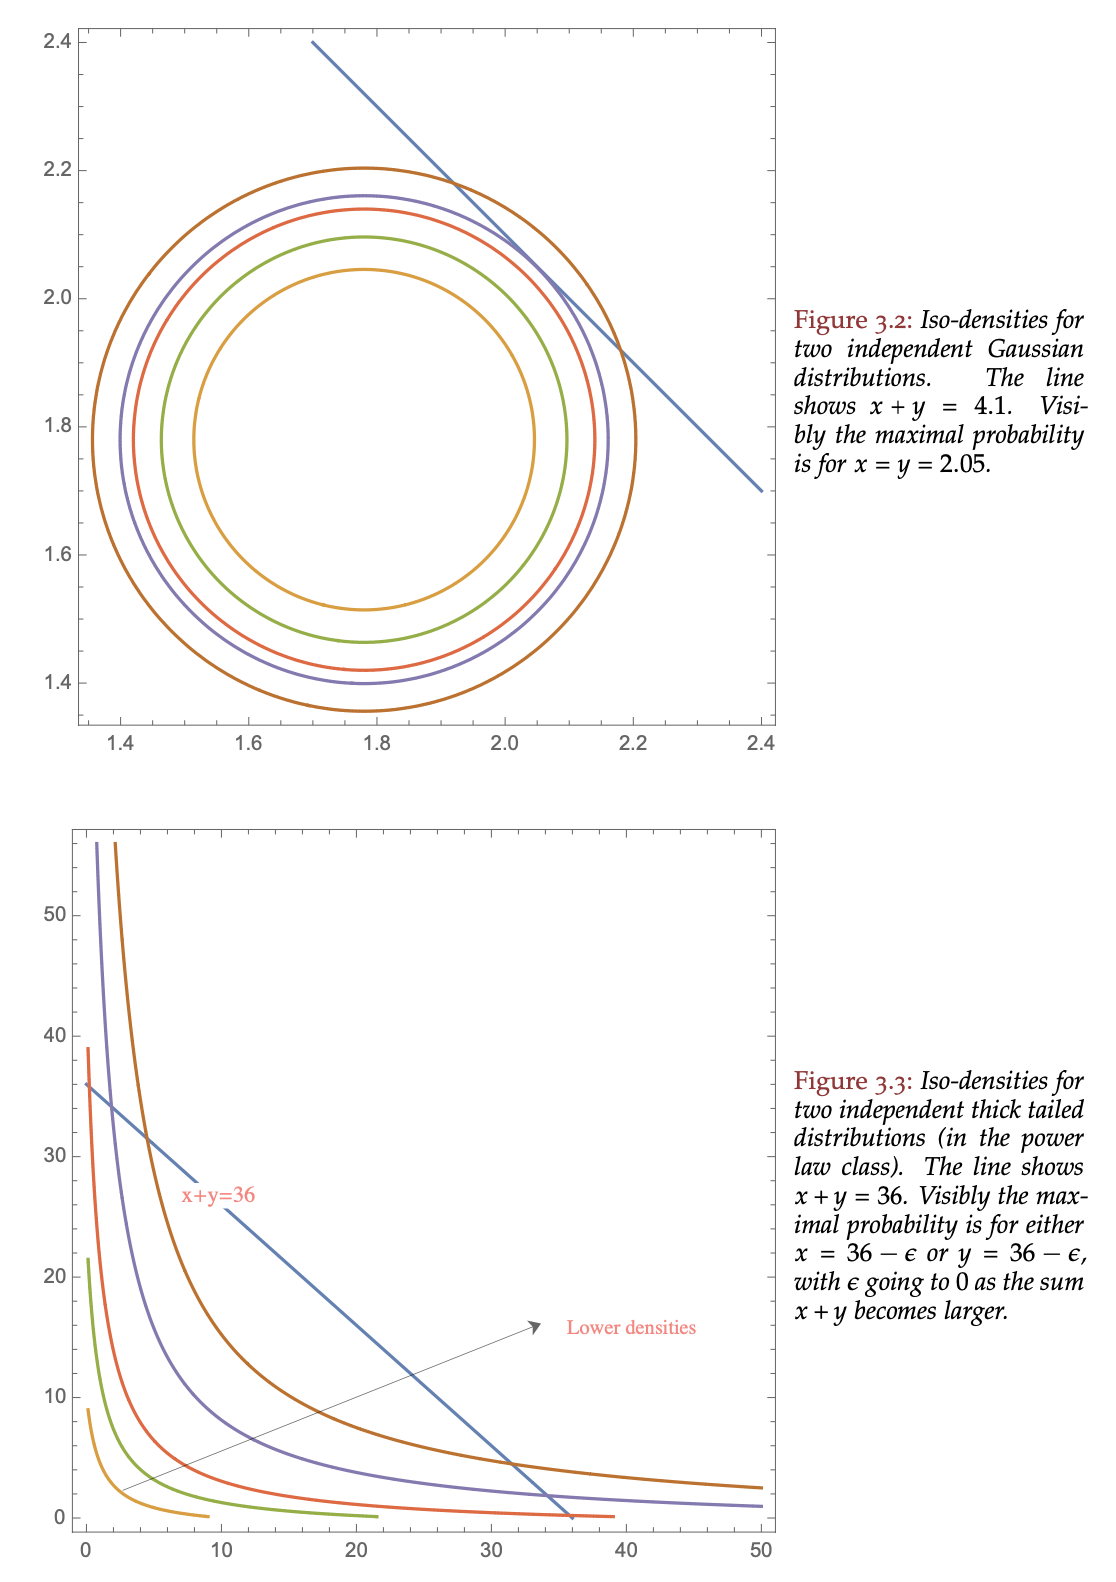
\includegraphics[width=\textwidth]{fattails01.png}
    \caption{Probability densities of two independent thin tailed and thick tailed random variables (brazenly copied from Taleb, 2020). Compare to plot of Lp norms. For the thin tailed random variables, the observa- tion of a particular sum is most likely to result from a balanced contribution from both random variables. For the fat tailed random variables, the observation of a particular sum is most likely to result from the contribution of one of the variables.}
    \label{fig:fattails01}
\end{figure}

\subsection{Consequences of Fat Tails}

\begin{figure}
\centering
    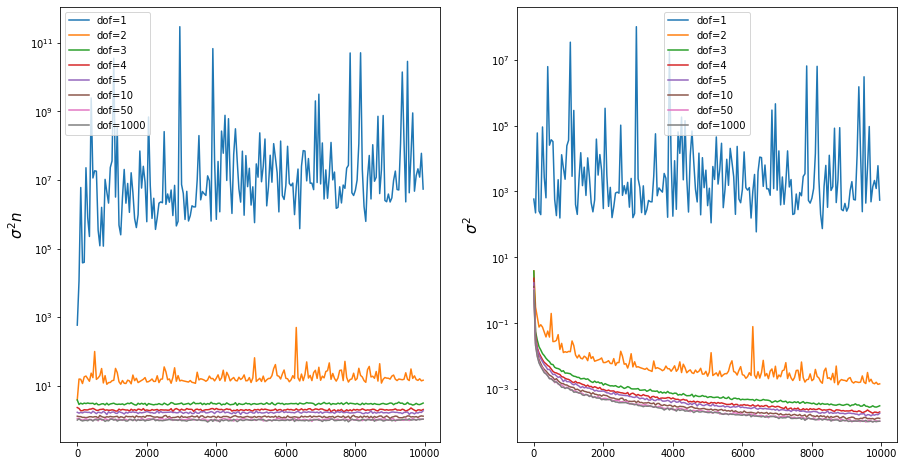
\includegraphics[width=\textwidth]{fattailsstudentt01.png}
    \caption{Probability densities of two independent thin tailed and thick tailed random variables (brazenly copied from Taleb, 2020). Compare to plot of Lp norms. For the thin tailed random variables, the observa- tion of a particular sum is most likely to result from a balanced contribution from both random variables. For the fat tailed random variables, the observation of a particular sum is most likely to result from the contribution of one of the variables.}
    \label{fig:fattails01}
\end{figure}

\begin{figure}
\centering
    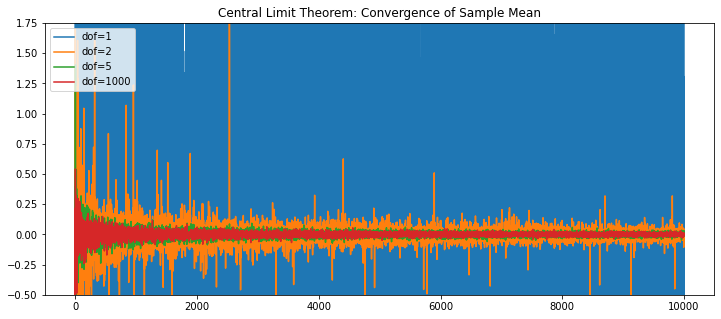
\includegraphics[width=\textwidth]{fattailstudentt02.png}
    \caption{Probability densities of two independent thin tailed and thick tailed random variables (brazenly copied from Taleb, 2020). Compare to plot of Lp norms. For the thin tailed random variables, the observa- tion of a particular sum is most likely to result from a balanced contribution from both random variables. For the fat tailed random variables, the observation of a particular sum is most likely to result from the contribution of one of the variables.}
    \label{fig:fattails01}
\end{figure}

\subparagraph{The Law of Large Numbers works too Slowly}

\subparagraph{The Sample Mean will rarely correspond to the Distribution Mean}
For example, for an 80/20 power law, 92\% of the observations will fall below the distribution mean. The sample mean will tend to underestimate the distribution mean because the distribution mean is heavily biased by rare observations that will tend to be underrepresented in the sample.

\subparagraph{Metrics such as Sample Mean and Sample Variance will be Unusable}

\subparagraph{In finance, metrics like Sharp etc. are unusable}

\subparagraph{Gauss-Markov Theorem fails}
Therefore, linear least squares regressions do not work. 

\subparagraph{Maximum Likelihood Methods can still work}
For example in case of a Pareto distribution, it is possible to fit the tail exponent using maximum likelihood methods, and estimating the mean from there. Direct observation of the mean would be misleading. The tail exponent intelligently extrapolates the fat tails of the distribution.

\subparagraph{Absence of Evidence $\neq$ Evidence of Absence}

\subparagraph{PCA is going to cause spurious factors and loads}

\subparagraph{Method of Moments does not work}
Approximating a distribution by matching its moments does not work when higher moments are undefined or cannot be reliably estimated.

\subparagraph{There is no ``typical" large deviation}


\subsection{Maximum to Sum}
The "maximum to sum" or MS plot allows to see the behavior of the relationship between the observed maximum to the sum for a particular moment as the number of observations increases. 

\subsection{Maximum Domain of Attraction}

The ``maximum domain of attraciton" is, so to speak, the ``right endpoint of the distribution":

\begin{equation}
x^* = \sup\{x: F(x) < 1 \}
\end{equation}

\subsection{Hidden Tail, Problems in Estimating Moments}
The Glivenko-Cantelli theorem guarantees uniform convergence of the empiral cdf to the true CDF, however, the empirical distribution is necessarily bounded by the values of the minimum and maximum observations. This results in an unobserved contribution to moments $p>0$ that does not necessarily have to be negligible. To illustrate, take $K_n$ to be the maximum observed value. 
\begin{equation}
\mathbb{E}(X^p) = \underbrace{\int_{L}^{K_n} x^p \phi(x)\mathrm{d}x}_{observed} + \underbrace{\int_{K_n}^{\infty} x^p \phi(x)\mathrm{d}x}_{unobserved}
\end{equation}


